%!TEX root = ../diplom.tex

\section{Моделирование процесса измерения}



При малых углах падения механизм обратного  рассеяния является квазизеркальным
и отражение происходит на участках волнового профиля, ориентированных
перпендикулярно падающему излучению. Тогда в формировании отраженного сигнала
будут участвовать только площадки, ориентированные нормально к излучению. 

\begin{figure}[h]
    \centering
    \begin{subfigure}{0.65\linewidth}
        \centering
        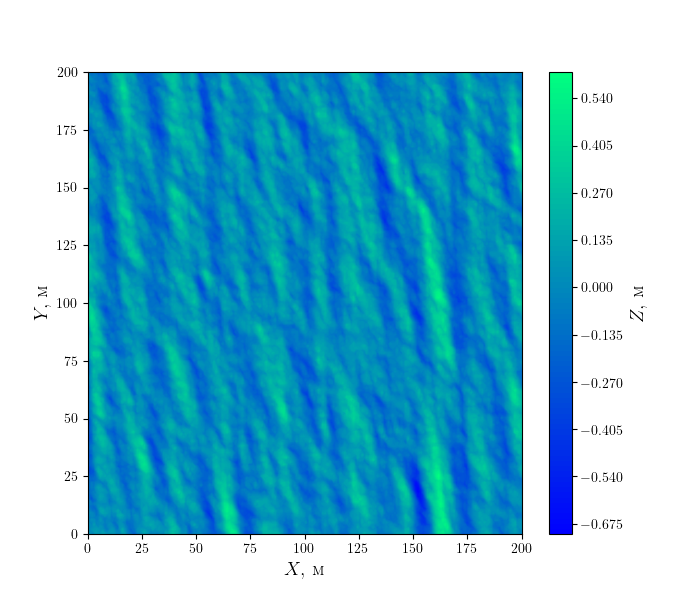
\includegraphics[width=\linewidth]{fig/impulse/fig1}
        \caption{Моделирование поверхности при скорости ветра $U=5$ м/с}
        \label{fig:mirror:a}
    \end{subfigure}
    \begin{subfigure}{.49\linewidth}
        \centering
        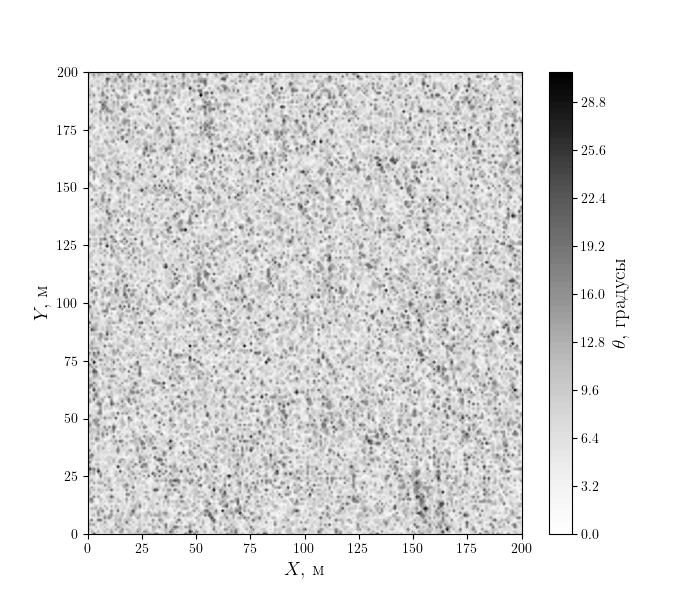
\includegraphics[width=\linewidth]{fig/impulse/fig2}
        \caption{Локальный угол отражения от поверхности для радиолокатора
        находящегося на высоте $H=1000$ км в точке с координатой (100, 100)}
        \label{fig:mirror:b}
    \end{subfigure}
    \begin{subfigure}{.49\linewidth}
        \centering
        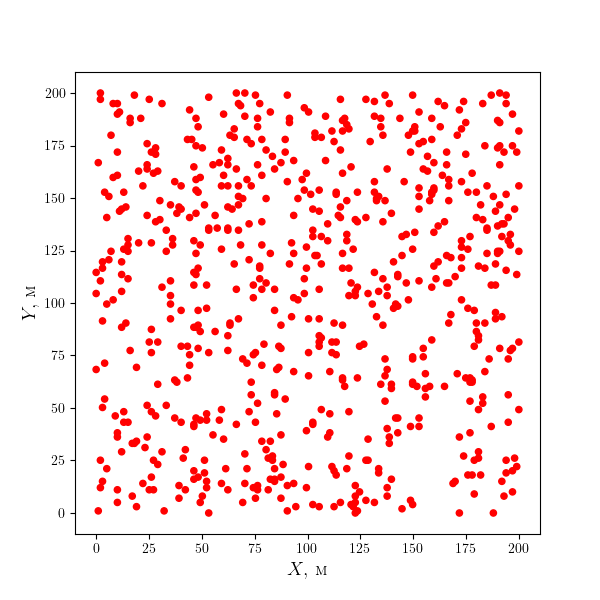
\includegraphics[width=\linewidth]{fig/impulse/fig3}
        \caption{Положение зеркальных точек поверхности \ref{fig:mirror:a} для
        радиолокатора находящегося над точкой (100,100) }
        \label{fig:mirror:c}
    \end{subfigure}
\end{figure}
